\documentclass{article}
\usepackage{graphicx}
\begin{document}
\huge
\textbf{Euler-Maruyama method}
\normalsize
\\

We want to find a way to solve stochastic ODEs numerically, which means finding a way to find the value of the function we want to find ($u_n$) at a certain point in time ($t_n$). 

For example, we can consider the \textbf{Geometric Brownian Motion} of the form

\[du = ru(t)\,dt + \sigma u(t) \,dW(t), \quad u(0)=u_0\]

Which has explicit solution \[u(t) = u_0\,e^{\left(r-\frac{\sigma^2}{2}\right)+\sigma W(t)}, \quad W(t)\sim \mathcal{N}(0,t)\].

We can find an approximate solution using a \textit{numerical method} called \textbf{Euler-Maruyama}, where \[u_{n+1} = u_n+ru_n\,\Delta t + \sigma u_n \,\Delta W_n, \quad W_n \sim \mathcal{N}(0,\Delta t)\]

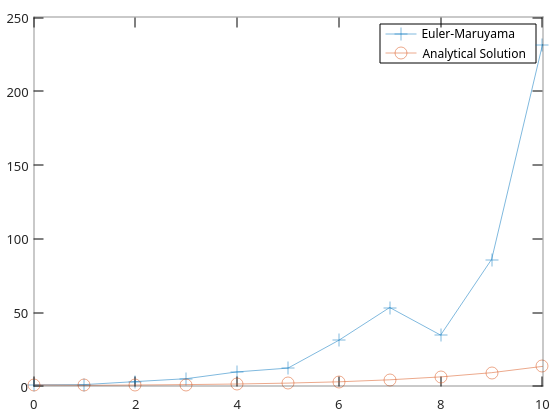
\includegraphics{./pic1}

But sometimes it doesn't work!
\\

So we introduce an improved version, called \textbf{Theta-Euler-Maruyama}: \[u_{n+1} = u_n + \left[(1-\theta)ru_n+(\theta) ru_{n+1}\right]\,\Delta t + \sigma u_n \,\Delta W_n, \quad W_n \sim \mathcal{N}(0,\Delta t)\]

and this always works well (for selected values of $\theta$).

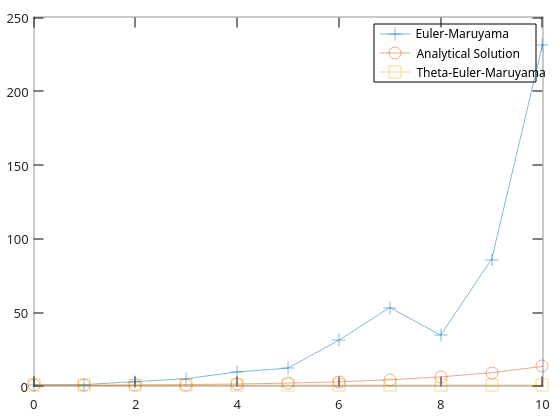
\includegraphics{./pic2}

\end{document}